\documentclass{article}

\usepackage{graphicx}
\usepackage{color,soul} % Highlighting
\usepackage{hyperref} % Clickable references
\usepackage{fancyhdr} % Header and footer
\usepackage{multirow}


\graphicspath{{./pic/}}

\begin{document}

\pagestyle{fancy}
\fancyhead{}
%\fancyhead[RO]{
\includegraphics[scale=0.03]{szines_SZTAKI_hunren_transzparens.png}}
\fancyhead[RO]{
\includegraphics[width=\textwidth]{header-crop.pdf}}
\renewcommand{\headrulewidth}{0pt}
\fancyfoot[LO]{
\includegraphics[width=\textwidth]{line.png} \\
\scriptsize
COPROLOGS – A projekt azonosítója: TKP2021-NKTA-01 \\
Kooperatív gyártó- és logisztikai rendszerek kutatása a versenyképes és fenntartható gazdaság \\
támogatására
}
\fancypagestyle{titlep}{%
	\fancyhead{}
	\fancyfoot[LO]{
\includegraphics[width=\textwidth]{line.png} \\
	\scriptsize
	COPROLOGS – A projekt azonosítója: TKP2021-NKTA-01 \\
	Kooperatív gyártó- és logisztikai rendszerek kutatása a versenyképes és fenntartható gazdaság \\
	támogatására
	}
}

\begin{titlepage}
	\thispagestyle{titlep}
   %\begin{center}
	   
\includegraphics[width=\textwidth]{header-crop.pdf}
       \vspace*{1cm}
       
       \begin{tabular}{lr}
    	   \multirow{5}{0.35\textwidth}{
\includegraphics{logo.png}} & {\small Kooperatív gyártó- és logisztikai rendszerek kutatása} \\
			& {\small a versenyképes és fenntartható gazdaság} \\
			& {\small támogatására} \\[2mm]
			& {\scriptsize A projekt azonosítója: TKP2021-NKTA-01} \\
			& {\scriptsize A projekt weblapja: \href{https://coprologs.eu}{https://coprologs.eu}} \\
       \end{tabular}
        \vspace*{3cm}

		\noindent
       \textbf{{\LARGE C3 -- Hálózati szimulációs környezet kidolgozása}}

       \vspace{0.5cm}
       \noindent
        {\Large Circular Supply Network Simulation Specification}
            
       \vspace{1cm}
       
       %\hrule
       \noindent
       
\includegraphics[width=\textwidth]{line.png}
       
       \vspace*{1cm}
       \noindent
       \begin{tabular}{ll}
       		Author: & Egri Péter \\
       		Reviewer: & Egri Péter \\
       		Date: & 2023.12.08 \\       
       \end{tabular}


       \vfill
            
       %\vspace{0.8cm}

		\noindent
       \begin{tabular}{lr}
       		{\scriptsize A projekt megvalósítója: SZTAKI} & \multirow{5}{0.35\textwidth}{
\includegraphics[width=0.4\textwidth]{nkfi.png}} \\
			{\scriptsize Székhely: 1111 Budapest, Kende utca 13-17.} & \\
			{\scriptsize Telefon: +36 1 279 6000} & \\
			{\scriptsize Weblap: \href{www.sztaki.hu}{www.sztaki.hu}} & \\
			&\\[4mm]
			
\includegraphics[height=6mm]{sztaki.png} 
\includegraphics[height=6mm]{epic.png} & \\
       \end{tabular}
\end{titlepage}

\title{
\includegraphics[scale=0.08]{szines_SZTAKI_hunren_transzparens.png} \\[1cm] Coprologs\footnote{TKP2021-NKTA-01} ~C3 Circular Supply Network Simulation Specification}
\author{Institute for Computer Science and Control (SZTAKI) \\ Research Laboratory on Engineering \& Management Intelligence}
%\author{P\'eter Egri}
%\date{December 2023}
%\maketitle

\newpage
\tableofcontents
\newpage

\section{Scope of the simulation}

\begin{itemize}
\item The focus is on \textbf{high level} (strategic, tactical) tasks. The simulation is aimed to be generic, therefore it will enable the development of \textbf{less detailed, general models}, focusing more on different types of \textbf{uncertainties}. This implies that resources will not be represented on detailed level (e.g., machines, labor) and the production capacities will be aggregated to factory level.
\item The simulation will take into consideration the \textbf{dynamic} nature of the \textbf{network structure} which can changes during runtime.
\item An important aspect of the simulation is the \textbf{circular economy} approach, which means considering the highly uncertain waste production of the consumers and modeling reverse logistic flows (e.g., reworking plants).
\item The simulation will be able to evaluate the resilience of the network, which necessitates the modeling uncertainties both in form of \textbf{stochastic behavior} and \textbf{sudden disturbances}.
\item The simulation will measure multiple \textbf{Key Performance Indicators} (KPI), such as financial (e.g., cost, profit), customer service (e.g., service level, lead time), and environmental (e.g., CO2 equivalent emission).
\item The simulation will also include the \textbf{energy consumption} of production, transportation and storage (e.g., refrigeration), in order to consider also the Greenhouse Gas (GHG) Protocol Scope 2 (indirect) emissions.
\item The simulation will include some \textbf{basic planning algorithms} in a modular way, thus it will enable the development and experiments with new algorithms.
\end{itemize}


\section{Case studies}

Since the Coprologs project does not involve any industrial partners, the requirements specification is based on past industrial case studies. Thus this specification is built both on real life requirements and their generalization in order to enable analyzing a wide scope of network problems using simulation. This section summarizes the most relevant case studies.


\subsection{Dynamic Network Optimization}

Dynamic Network Optimization (DNO) was a simulation project for analyzing and optimizing an international distribution network. Since the focus was on the \textbf{distribution}, only the \textbf{finished product} were considered, therefore the details related to production were not considered. That means, no suppliers, materials and BOMs were considered in the simulation.

The nodes of the network were a \textbf{central distribution center} in Asia, one existing and several potential \textbf{local distribution centers} in Europe, and \textbf{several customer locations} also in Europe.

The \textbf{demand} of the customers were given by historical data, which allowed to experiment with different transportation modes and distribution routes for serving the customers, as well as to analyze the demand patterns and generate realistic demand scenarios. All demand had to be served, but transportation to the local distribution centers could be made without customer demand, in order to \textbf{build inventories} and/or to \textbf{fill transportation capacity}. The customer demands were distinguished by their service level, which could be \textbf{standard} or \textbf{expedite shipping}.

Several \textbf{transportation modes} were considered in the model, which were different in their speed, cost, capacity and route limitations. Basically, from the central distribution center to the local ones two options were allowed: ocean and air transportation. Serving the customers from local distribution centers was limited only to truck delivery. Alternatively, customers could be served directly from the central distribution center by parcel couriers.

The goal of the project was to provide a tool for performing \textbf{what-if analysis} of the distribution and transportation logic of the network. The main performance indicator was the transportation cost, but several other statistics were calculated also, e.g., inventory levels or identifying the key customers.

We designed and developed a modular simulation system for analyzing the described problem, see Fig.~\ref{fig:dno}. The main components of the system are the simulation model and engine, the consolidation logic module and the demand generator module. The simulation is responsible for executing the given transportations, calculating performance indicators, as well as providing graphical representation of the distribution network and general user interface. The consolidation logic is responsible for planning the transportation based on the customer demand. The implemented logic is quite complex, and it can be externally parameterized in order to create and analyze different scenarios. Finally, the demand generator module analyzed the historical demand, recognized demand patterns and created future orders accordingly. The consolidation and demand generator modules were implemented as external module libraries that were executed by the main simulation component.

\begin{figure}[ht!]
	\center
	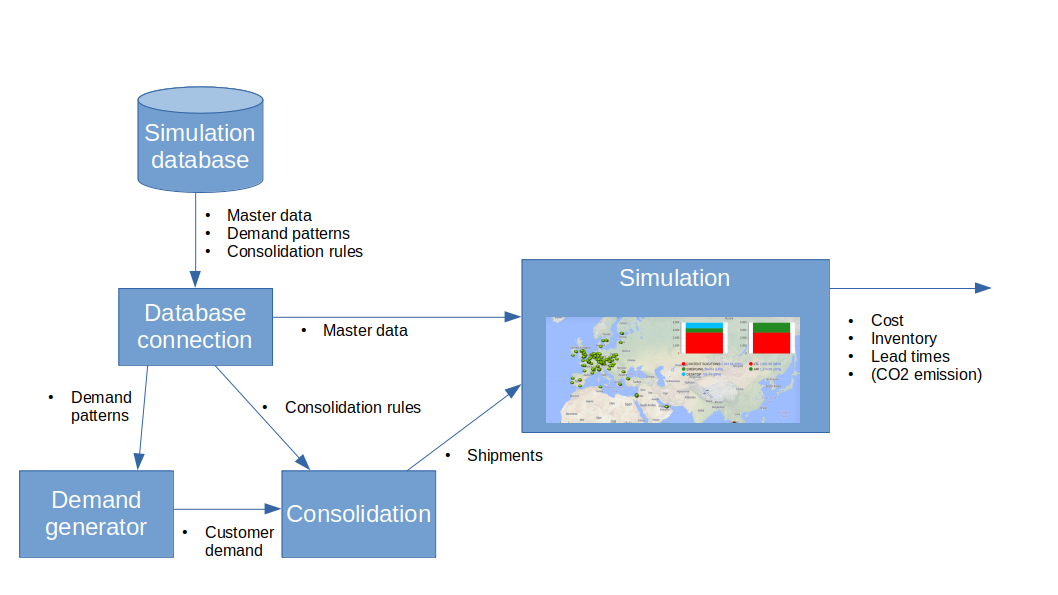
\includegraphics[width=\textwidth]{dno.png} 
	\caption{Architecture of the DNO system}\label{fig:dno}
\end{figure}


\subsection{Battery production and recycling network}

%https://batteries.guide.digiprime.eu/

The battery network case study is related to \textbf{re-manufacturing} and \textbf{re-use} of second life Li-Ion battery (LIB) cells. The battery pack is the most important component of a hybrid and full electric vehicle, making up more than one third of the cost of the vehicle itself. Unavoidable chemical and physical degradation of the cells forces battery packs to a performance fade over time. These battery packs have an \textbf{average lifespan of 8 to 10 years}, during which their actual capacity degrades below the 80\% of the initial capacity, requiring pack substitution.

Packs which are not anymore suitable for traction purposes preserve high value, since \textbf{aging and failure of cells is an uncertain process} and in post-use modules both strongly compromised cells as well as poorly degraded cells are found. Several solutions have been investigated to preserve post-use Li-Ion battery value, see Fig.~\ref{fig:digiprime}. The two most common approaches are (i) direct re-use of battery packs for stationary and non-stationary applications, and (ii) open loop recycling, i.e., to apply pyro-metallurgical processes for cobalt (and rarely lithium) recycling.


\begin{figure}[ht!]
	\center
	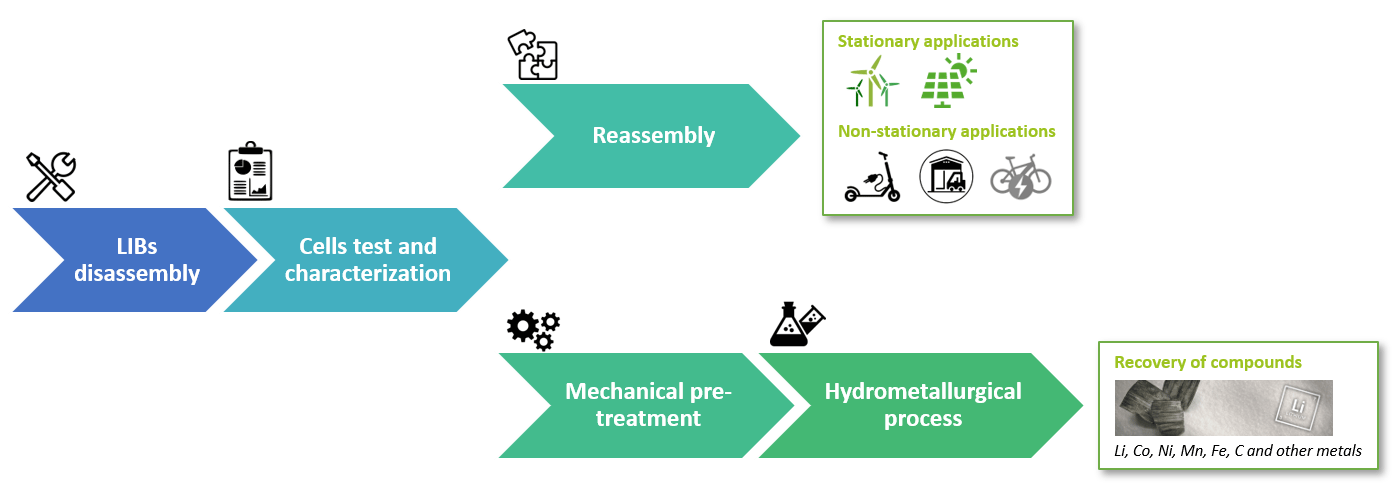
\includegraphics[width=\textwidth]{digiprime.png} 
	\caption{Reverse logistic chain of lithium-ion batteries (LIBs)}\label{fig:digiprime}
\end{figure}


\subsection{Router repair network}

This case study especially focuses on the \textbf{re-manufacturing} part of a telecommunications infrastructure production network. The main company is a global electronics repair and service provider having several sites in North and South America, Europe and East Asia. The other members of the network are the customers, the delivery companies and the router manufacturing service providers.

The products are returned in \textbf{high-mix, low-volume (HMLV)} and the network yield altogether over 2.5 million returned devices each year. Most of the products have \textbf{complex structures} consisting of printed circuit boards. In addition, several \textbf{products are localized} to a specific region. The repair company has different sites all over the world with \textbf{specialized knowledge} on certain products, therefore selecting the right location is of utmost importance for high-quality service.


The \textbf{defected products} returned to the repair company \textbf{should be replaced} with either a new, a repaired or a or re-manufactured product. The defected routers should be also repaired or re-manufactured for further use. The repair process starts with the identification of the error and continues with the replacement and/or repair of the broken part. The production \textbf{lead time is highly variable} and dependent on the initial product status.


\section{Overview of related supply chain simulation systems}

There are several commercial and open source computer simulation software, some of them are specialized to simulate supply chain and logistics networks. In this section, we briefly overview the most relevant tools.


\subsection[AnyLogistix]{AnyLogistix\protect\footnote{\href{https://www.anylogistix.com/}{https://www.anylogistix.com/}}}

AnyLogistix is the most relevant general simulation and optimization software for supply chains. Its functionalities are: green field analysis (supply network facility location problem), network optimization (inventory and transportation optimization), production (transportation, inventory and sourcing policy, considering bill-of-materials) and risk management (bullwhip- and ripple effect analysis).


\subsection[OTD-NET]{OTD-NET\protect\footnote{\href{https://www.iml.fraunhofer.de/en/fields_of_activity/enterprise-logistics/supply\_chain_engineering/products/otd-net.html}{https://www.iml.fraunhofer.de/en/fields\_of\_activity/enterprise-logistics/supply\_chain\_engineering/products/otd-net.html}}}

The OTD-NET (Order-to-Delivery Network) is a proprietary simulation system for modeling and simulating production networks being developed by Fraunhofer IML, mainly focusing on the automotive sector applications. Few information is available online, a screenshot with the network elements can be seen in Fig.~\ref{fig:otdnet}.

\begin{figure}[ht!]
	\center
	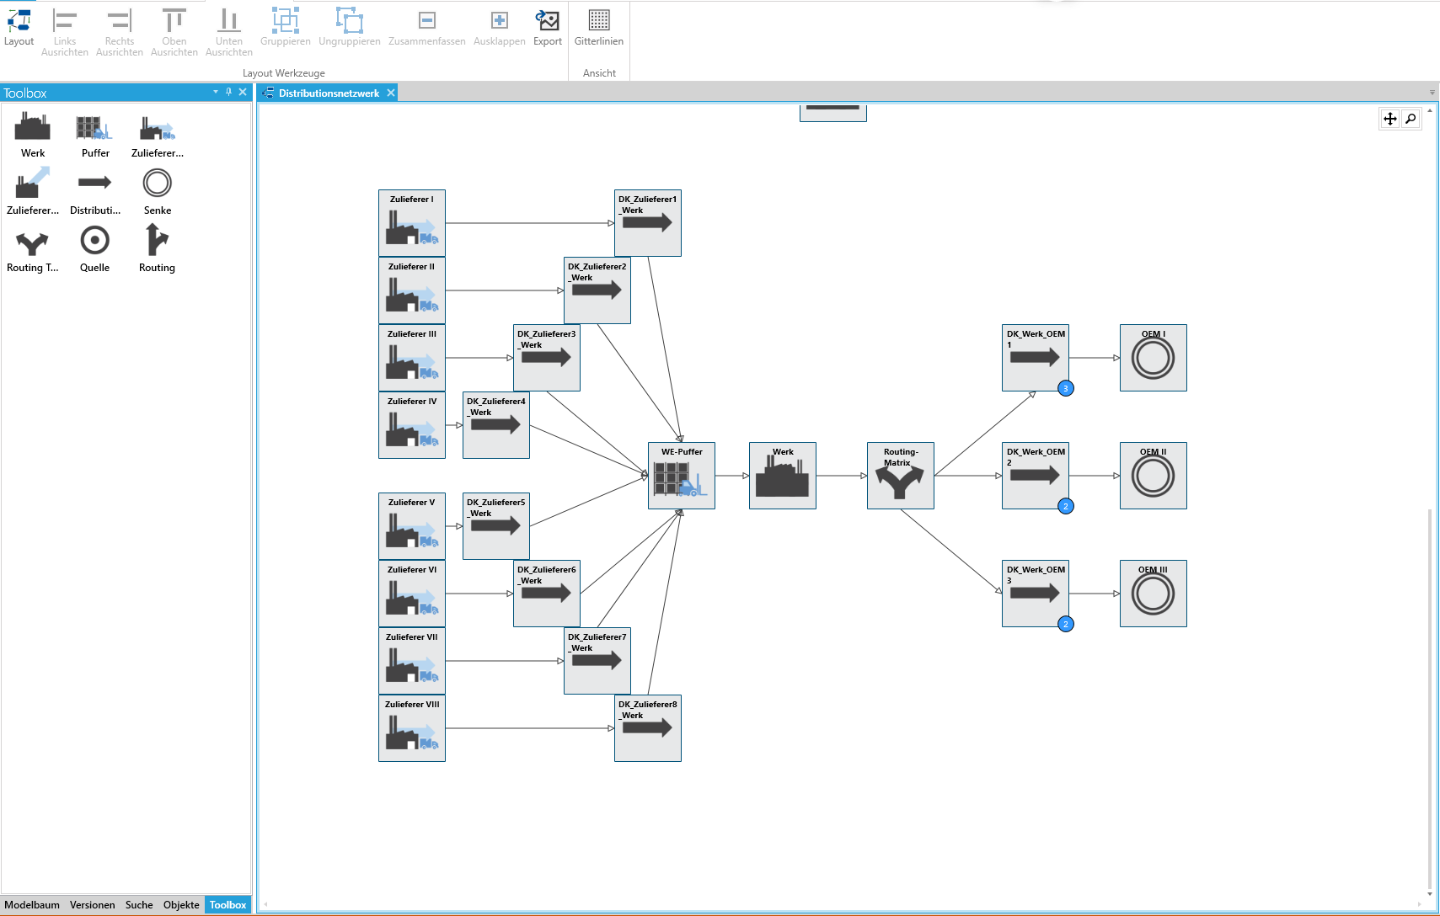
\includegraphics[width=.7\textwidth]{otdnet.png} 
	\caption{OTD-NET interface}\label{fig:otdnet}
\end{figure}


\subsection[SCM Globe]{SCM Globe\protect\footnote{\href{https://www.scmglobe.com}{https://www.scmglobe.com}}}

SCM Globe is a cloud-based supply chain simulation tool. The four main elements of the model are: products, facilities, vehicles and routes, see Fig.~\ref{fig:scmglobe}.

\begin{figure}[ht!]
	\center
	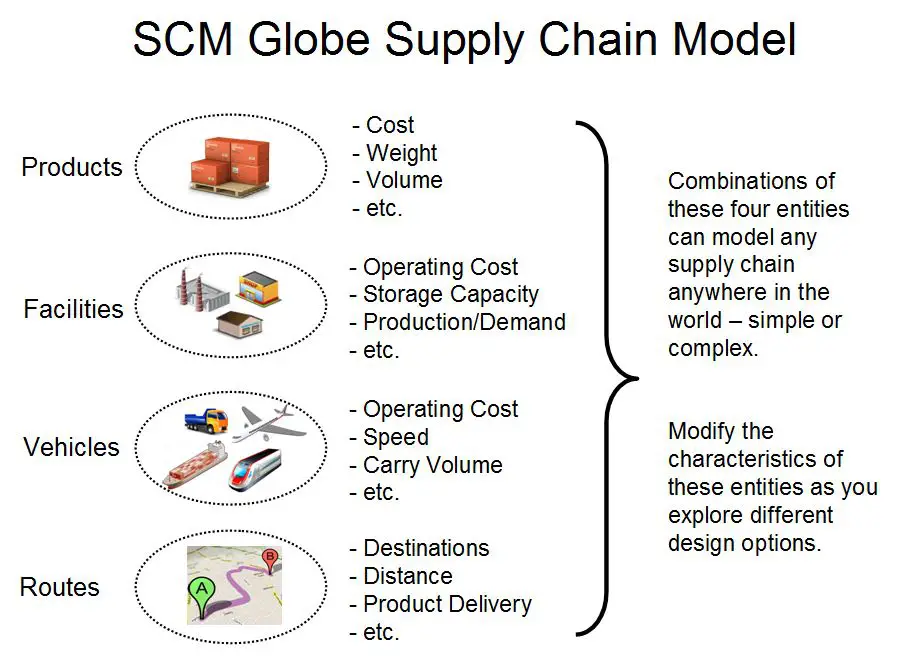
\includegraphics[width=.7\textwidth]{scmglobe.png} 
	\caption{Components of the SCM Globe toolkit}\label{fig:scmglobe}
\end{figure}


\subsection[AnyLogic]{AnyLogic\protect\footnote{\href{https://www.anylogic.com}{https://www.anylogic.com}}}

AnyLogic is a general multimethod simulation tool that can be used for building various types of simulation models, including supply chain simulations.

Since SZTAKI has both the licence and experience with AnyLogic, this seems to be the most appropriate candidate to be used for developing the circular network simulation in the Coprologs project.


\subsection[FlexSim]{FlexSim\protect\footnote{\href{https://www.flexsim.com/supply-chain-simulation}{https://www.flexsim.com/supply-chain-simulation}}}

FlexSim is another general purpose simulation tool using discrete event simulation method.

\subsection[Arena]{Arena\protect\footnote{\href{https://www.rockwellautomation.com/en-us/products/software/arena-simulation/discrete-event-modeling/supply-chain.html}{https://www.rockwellautomation.com/en-us/products/software/arena-simulation/discrete-event-modeling/supply-chain.html}}}

Arena is also a general purpose simulation tool using discrete event simulation method. According to its description, it is capable modeling JIT operations, evaluating transportation alternatives, optimizing facility location, evaluating dispatching rules, planning facility sizes, identifying bottlenecks, quantifying risks, determining warehouse capacities, evaluating warehouse picking strategies and determining labor requirements.


\section{Supply network simulation description}

The goal of the supply network simulation system is to evaluate the high-level, long-term behavior of the network, therefore the model considers general structures and decisions, while disregards operational details.

The basic concept of a circular supply chain network can be seen in Fig.~\ref{fig:circular}. The production process goes through a chain of production plants until the end customer. At the end of the product service life, the product can be returned to the network, where a recovery plant disassembles the product to the largest reusable parts and transports them back to the supply chain according to the demand. The results of this disassembly is stochastic due to the uncertain condition of the waste product.

\begin{figure}[ht!]
	\center
	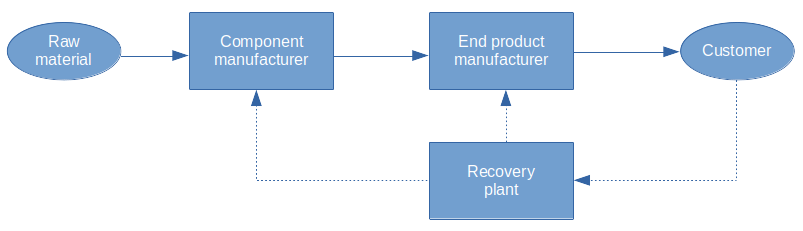
\includegraphics[width=\textwidth]{circular.png} 
	\caption{Basic structure of a circular supply chain}\label{fig:circular}
\end{figure}

\subsection{Material}

Materials represent both components and finished products produced by the network nodes. Materials have a \textbf{volume} per unit property, which is used to calculate the occupied space of the materials in the warehouses in order to respect their capacity limits. %Volume is also used to calculate the transportation cost between nodes.

Materials can be raw materials which do not have any components, otherwise they consist of components defined by the \textbf{bill-of-materials (BOMs)}.

If the components of the material can be reused, the disassembly structure is described by and \textbf{inverse BOM}, which can be a sub-graph of the material’s BOM.

\subsection{Network node} \label{sec:node}

The network nodes represent customers (or markets), production and recovery plants, as well as distribution and collection centers of the network. Each node’s \textbf{location} is given by the geographic coordinates. Due to the dynamic nature of the networks, the existence of the nodes are specified by \textbf{calendars}. There can be \textbf{initial inventories} specified for each nodes at the beginning of the simulation run.

\subsubsection{Customer}

Customers purchase materials (mainly finished products) with stochastic \textbf{demand}. Customers also generate \textbf{waste} materials, which may be collected and reused in the network after recovery.

\subsubsection{Production plant}

Production plants make or assemble specific \textbf{materials} described by their BOMs, up to their \textbf{capacity} levels. Production of a material is characterized by its \textbf{cost}, \textbf{time} and \textbf{capacity usage}. The produced materials are sold at some \textbf{price}.

\subsubsection{Distribution center}

A distribution center stores materials up to its \textbf{capacity}.

\subsubsection{Collection center}

Collection centers stores waste products collected from customers until they are sent to recovery plants. Similarly to distribution centers, a collection center has storage \textbf{capacity}.

\subsubsection{Recovery plant}

Recovery plants disassemble used products into its components. The disassembly is described by an \textbf{inverse BOM}, and also characterized by its \textbf{cost}, \textbf{time} and \textbf{capacity usage}. Due to the uncertain quality of the used products, the \textbf{quantities} of the resulted components are stochastic.


\subsection{Transport mode} \label{sec:transport_mode}

Transport mode describes the material transportation between nodes. Different modes (truck, rail, air, ship) provide different transportation \textbf{cost} and \textbf{time}. The cost can be further divided into \textbf{fixed cost} (e.g., vehicle maintenance, amortization, driver personnel) and distance-based \textbf{variable cost}. Not every mode can be used in all situations, for each pair of nodes there are different \textbf{possible transport modes}. The typical transport modes are:

\begin{itemize}
\item Ocean: slow and inexpensive transportation mode, limited to long (intercontinental) distances.
\item Air: fast and expensive transportation mode, mainly for long distances.
\item Truck: relatively fast transportation mode, mainly for short and medium distances. It is also relatively expensive due to high fuel prices. This is the most commonly used transportation mode in the distribution and therefore huge percentage of the transportation cost and transportation CO2 emission is caused by truck delivery.
\item Rail: slower and cheaper transportation mode than the truck delivery, mainly for medium and long distances. Availability restrictions may apply.
\item Parcel: the fastest and most expensive transportation mode, it is used mainly for special expedite deliveries.
\end{itemize}

\subsection{Cost center}

Cost centers are distinct parts of the network, typically nodes and transportation belonging to different companies. With these logical entities, the occurred costs, profits and other KPIs can be summarized on company level. Typical KPIs are including:

\begin{itemize}
\item Production and transportation costs,
\item Production and transportation emissions,
\item Provided lead-times for the customers,
\item Number and volume of lost sales,
\item Production capacity utilization, and
\item Average inventory levels.
\end{itemize}


\subsection{Disturbances}

Disturbances describes sudden problems in the network which are different from the typical fluctuations. Disturbance can happen at the production and recovery nodes, which means the node cannot operate (or operate with a reduced capacity) for a given period of time. Such a \textbf{node failure} causes delays in the network. There is also a possibility of \textbf{limited and/or long lead time supply}, due to raw material scarcity.

Failures can also occur at transportation time. Besides \textbf{delays} in transportation, the shipment can even be \textbf{lost}, e.g., because of theft, sunken ship, etc.


\subsection{Business models}

A business model characterizes the relationship between two network nodes.

\subsubsection{Business-to-customer (B2C)}

The customers of the end products are usually served from distribution centers. Customers can decide for each product, if they accept \textbf{backlogs} when the ordered quantity is not available at the distribution center, otherwise the order becomes \textbf{lost sale}. For the potential \textbf{make-to-order} business models, the inventory target level is zero, therefore lost sales do not apply.


\subsubsection{Business-to-business (B2B)}

The supply relationship between two production sites is linked by two inventories: the finished good inventory (or distribution center) of the supplier and the component inventory of the buyer, see Fig.~\ref{fig:b2b}.

\begin{figure}[ht!]
	\center
	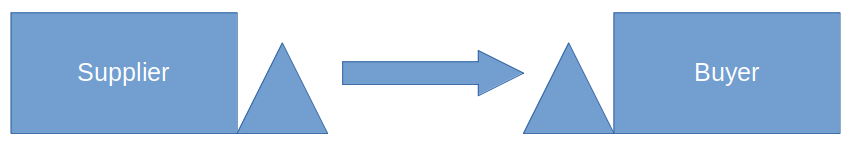
\includegraphics[width=\textwidth]{b2b.png} 
	\caption{Supply relationship between two nodes}\label{fig:b2b}
\end{figure}

The levels of these inventories are set by the inventory planning module, see Section \ref{sec:inventory}. Typical cases of the B2B relation are:

\begin{itemize}
\item The buyer holds component inventory, while the supplier only produces to orders.
\item The supplier holds inventory and serves the buyer from the inventory.
\item The supplier holds inventory at the buyer's site (\textbf{vendor managed inventory} (VMI)).
\item Neither partners hold inventory, production is made in a completely \textbf{pull system}.
\end{itemize}


\section{Decision modules}

The simulation system will facilitate experiments with different planning algorithms. Therefore some substantial decision tasks will be built in a modular way, in order to enable the extension of the simulation with novel algorithms developed as external modules. The system will include the following decision modules.

\subsection{Forecasting}

Estimates the future demand for materials. Some typical possibilities are:

\begin{itemize}
\item Moving average.
\item Exponential smoothing.
\end{itemize}

\noindent Required data:
\begin{itemize}
\item Past demand (date, quantity)
\end{itemize}

\begin{figure}[ht!]
	\center
	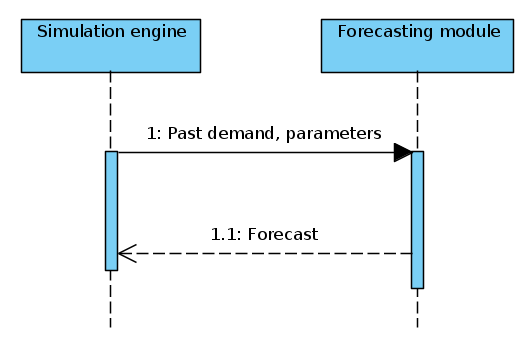
\includegraphics[width=.6\textwidth]{seq_fcst.png} 
	\caption{Forecasting}\label{fig:seq_fcst}
\end{figure}


\subsection{Supplier selection}

Whenever a material can be purchased from multiple suppliers, the supplier selection module decides which suppliers are chosen. Some typical possibilities are:
\begin{itemize}
\item Cheapest price.
\item Closest supplier.
\item Trustfulness (based on past performance).
\item Dual or multiple sourcing.
\item Other/combined approach.
\end{itemize}

\noindent Required data:
\begin{itemize}
\item Available suppliers (price, distance, past performance)
\end{itemize}

\begin{figure}[ht!]
	\center
	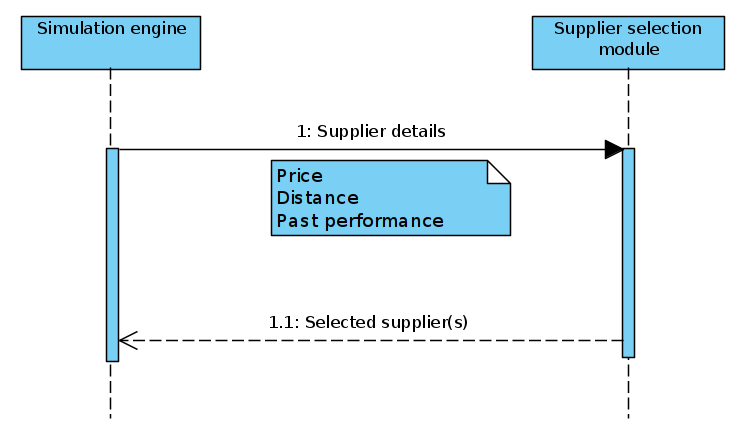
\includegraphics[width=.7\textwidth]{seq_supplier.png} 
	\caption{Supplier selection}\label{fig:seq_supplier}
\end{figure}


\subsection{Inventory planning/order lot sizing}\label{sec:inventory}

This module controls both the purchasing and production of the materials, including the computation of \textbf{order lot sizes}, \textbf{safety stocks} and \textbf{reorder points}. Different materials can use different rules. Some typical possibilities are:

\begin{itemize}
\item Forecast-based push system.
	\begin{itemize}
	\item Periodic inventory review.
	\item Continuous inventory review.
	\end{itemize}
\item Order-based pull system.
\end{itemize}

\noindent Required data:
\begin{itemize}
\item Past demand (date, quantity) -- for classifying materials
\item Inventory level (quantity)
\item Storage limit
\item Demand forecast (date, quantity)
\item Material price (amount)
\item Fixed ordering/transportation/production cost (amount)
\end{itemize}

\begin{figure}[ht!]
	\center
	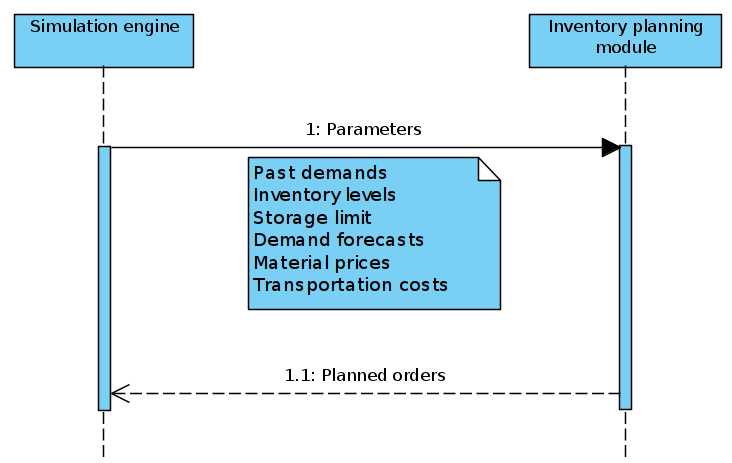
\includegraphics[width=.7\textwidth]{seq_inventory.png} 
	\caption{Inventory planning}\label{fig:seq_inventory}
\end{figure}


\subsection{Order processing}

Whenever a demanded material is not available in the demanded quantity and there are several orders, the dispatching logic should decide how to distribute the available materials among the orders. Some typical possibilities are:
\begin{itemize}
\item First come, first served (FCFS).
\item Largest order first.
\item Smallest order first.
\item Lost sale orders first, backlog orders later.
\item Best buyer first.
	\begin{itemize}
	\item According to annual order value.
	\item According to variety of ordered materials.
	\end{itemize}
\end{itemize}

\noindent Required data:
\begin{itemize}
\item Inventory level (quantity)
\item Orders (quantity, backlog allowance)
\item Past orders (date, quantity (or value))
\item Past provided service levels (lead times)
\end{itemize}

\begin{figure}[ht!]
	\center
	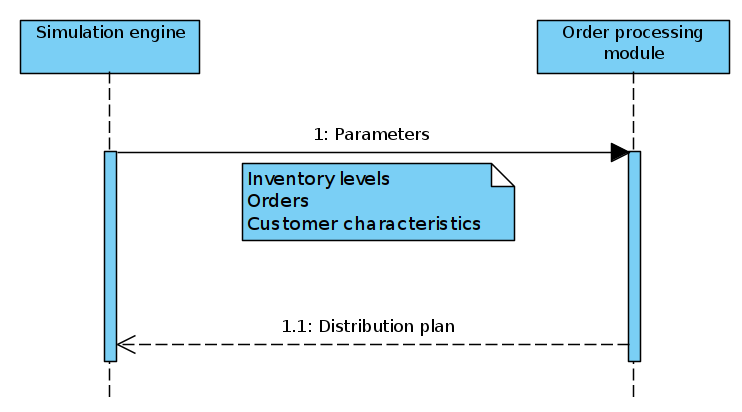
\includegraphics[width=.7\textwidth]{seq_dispatching.png} 
	\caption{Order processing}\label{fig:seq_dispatching}
\end{figure}


\section{Simulation architecture}

\begin{figure}[ht!]
	\center
	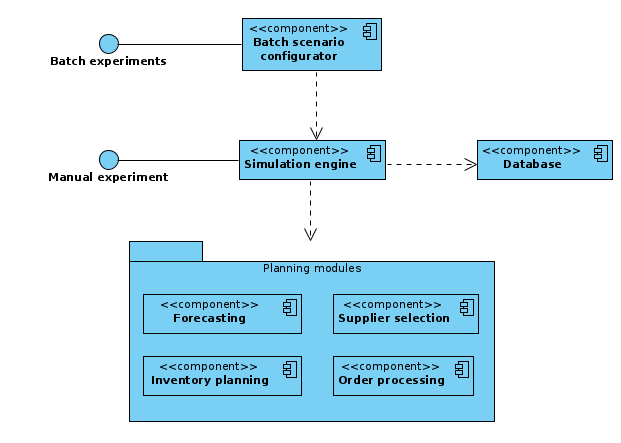
\includegraphics[width=\textwidth]{architecture.png} 
	\caption{Architecture of the simulation system}\label{fig:architecture}
\end{figure}

The overview of the system architecture with the main components and their dependencies is shown in Fig.~\ref{fig:architecture}. The main component is the \textbf{simulation engine} implemented in AnyLogic. The engine build the network model based on the configuration stored in a SQLite \textbf{database}, which is also used to store the results of the simulations. The \textbf{planning modules} used in the simulation are implemented in Java and stored as external JAR files which can be replaced or extended without modifying the other components. While the simulation engine can be used for manual experimentation, the \textbf{batch scenario configurator} will enable executing, evaluating and comparing multiple simulation with different parameters.

\subsection{Agents of the simulation system}

Agents will represent such objects in the model that have geographical locations, these are the \textbf{network nodes} and \textbf{transportation vehicles}. Both agent types will have several sub-types (see Sections \ref{sec:node} and \ref{sec:transport_mode}). Other objects of the model (materials, orders, etc.) will be defined by Java classes.


\section{Database structure}

The configuration of the supply chain network will stored in a relational database and read by the simulation engine. The data tables can be seen in Fig.~\ref{fig:datamodel}.

\begin{figure}[ht!]
	\center
	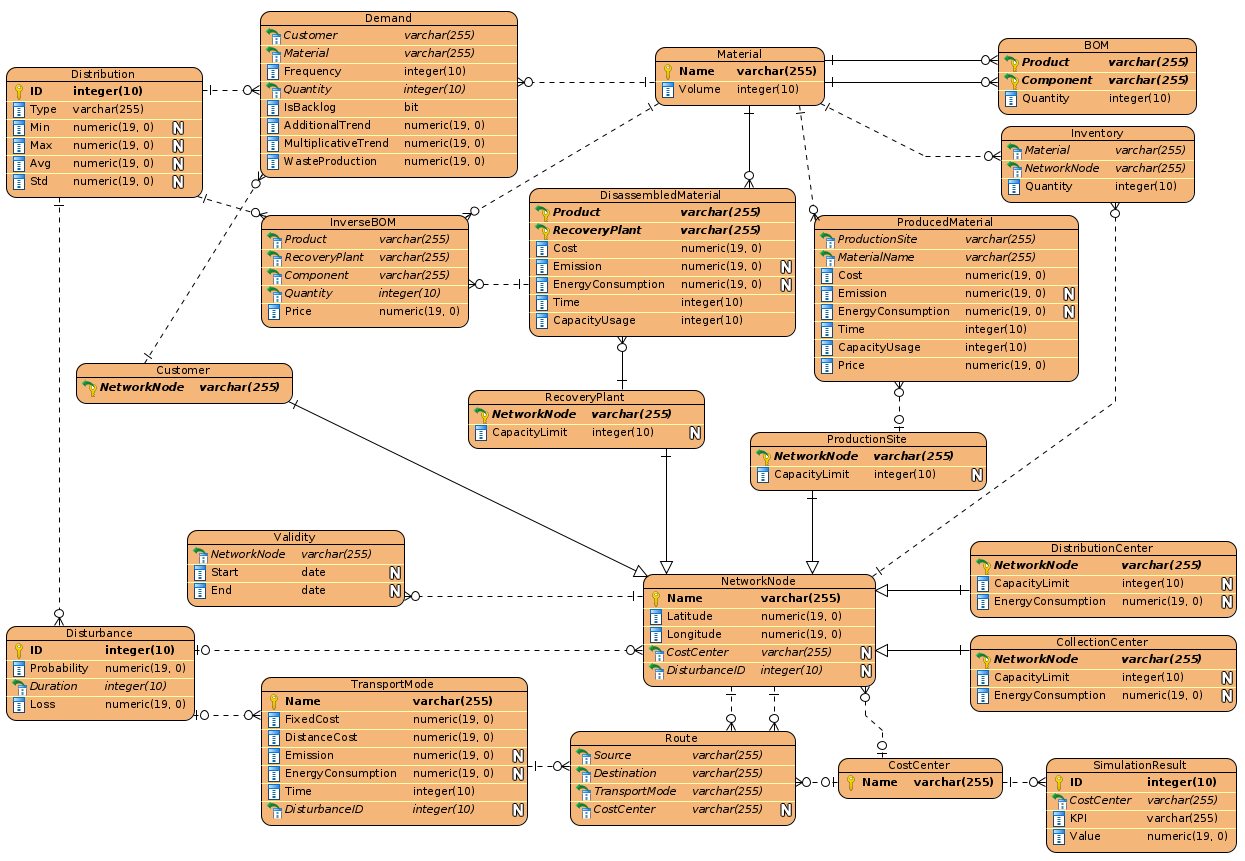
\includegraphics[height=\textwidth,angle=90,origin=c]{datamodel.png} 
	\caption{Database structure of the simulation system}\label{fig:datamodel}
\end{figure}

\subsection{Material (components, products)}

Materials are the primary flows in the supply network simulation.
\begin{itemize}
\item Volume: used for calculating the inventory size for respecting the capacity limits.
\item BOM: describes the required materials and quantities for the production.
\end{itemize}

\subsection{NetworkNode}

Nodes are the main components of the supply chain network. They can be of five sub-types: customer, production site, distribution center, collection center and recovery plant.

\begin{itemize}
\item Location: latitude and longitude of the node. The location is required for the distance estimation and also for the presentation.
\item Time: intervals when the node is working (can be open ended).
\end{itemize}
\begin{enumerate}
\item Customer
	\begin{itemize}
	\item Demand: characterized by the frequency, the distribution and whether the customer accepts backlogs when the demand cannot be shipped from the distribution center. Linearly and/or multiplicatively increasing or decreasing demand can also be specified with the additive and multiplicative trend parameters, respectively. This enables investigating the ramp-up and ramp-down phases.
	\item Waste: percentage of the used product returned for recovery.
	\end{itemize}
\item Production plant
	\begin{itemize}
	\item Capacity limit: production limit per time period.
	\item Produced materials: characterized by the production cost, production time, used capacity, CO2 equivalent emission, energy consumption and selling price.
	\end{itemize}
\item Distribution center
	\begin{itemize}
	\item Capacity limit in volume.
	\item Energy consumption: for storing materials.
	\end{itemize}
\item Collection center
	\begin{itemize}
	\item Capacity limit in volume.
	\item Energy consumption: for storing materials.
	\end{itemize}
\item Recovery plant
	\begin{itemize}
	\item Inverse BOM: describe the disassembly process of the waste products. It is characterized by the disassembly cost, time, used capacity, produced quantity (which is stochastic due to the uncertain quality of the waste), CO2 equivalent emission, energy consumption and selling price for each component.
	\end{itemize}
\end{enumerate}


\subsection{Transport mode}

\begin{itemize}
\item Fixed cost: e.g., driver salary, motorway vignette, etc.
\item Transportation cost: based on the traveled distance.
\item Transportation time: based on the traveled distance.
\item Emission: the CO2 equivalent emission of the transportation, based on the distance.
\item Energy consumption: based on the distance.
\end{itemize}


\subsection{Route}

Route describes an edge between a source and a destination node, specifying the used transport mode. There can be several alternative routes between the same pair of nodes using different transport modes.


\subsection{Distribution}

Statistical distribution describing the uncertain variables such as demand and recovered materials. It is characterized by the type of the distribution and with possible other parameters, such as minimum, maximum, average and standard deviation. Typical distributions:

\begin{itemize}
\item Uniform: given by the minimum and maximum values.
\item Triangular: given by the minimum, maximum and average values.
\item (Truncated) normal: given by the average and standard deviation values. If also the minimum and/or maximum values are given, then the distribution will be truncated, i.e., for avoiding negative demands.
\end{itemize}


\subsection{Disturbance}

Disturbances usually describe low probability, high impact problems at the network nodes or during transportation. They can be unexpected delays (e.g., breakdowns) and even products can be (partially) lost (e.g, due to theft).


\subsection{Cost centers}

Cost centers represent a company or a division, they may contain multiple nodes and routes. The computed KPIs are aggregated to cost center level.


\subsection{SimulationResult}

Simulation result records contain the resulted KPI-value pairs for each simulation run, aggregated to cost center level.


\section{Typical use cases}

The supply network simulation system will enable performing what-if analysis, experimenting, evaluating and comparing the results of different decisions. Some of the major use cases are listed below.

\subsection{Planning algorithms}

Due to the modularity of the system, the main planning algorithms can be replaced with customly developed external modules, which enables evaluating the application of different planning algorithms. For example, this enables evaluating the difference between applying single- or multi-sourcing, or using different transport modes.


\subsection{Facility location}

The user can specify different locations for production sites, distribution centers, collection centers and recovery plants, then run the corresponding simulation and compare the results.


\subsection{Scenario analysis}

The simulation system also enables the evaluation of different possible future scenarios, such as increased oil prices, more scarce materials, decreased labor supply, decreased demand due to a new competitor or increased number of disturbances in the network.


\subsection{New product introduction/ramp-up or ramp-down}

Typical situations in production networks include the increasing demand during a new product introduction and the decreasing demand during the ramp-down phase. In both cases special attention is required in order to balance between the service, the cost and the inventory related KPIs.


\end{document}